\documentclass{beamer} 			
\usepackage[utf8]{inputenc} 
\usepackage[T1]{fontenc}	
\usepackage{lmodern}		
\usepackage[english]{babel}		
\usepackage{amsmath}
\usepackage{amsfonts}
\usepackage{amssymb}
\usepackage{comment}	
\usepackage{epstopdf} 	
\usepackage{bookman}
\usepackage{xcolor}
\usetheme{CambridgeUS}	
\usecolortheme{beaver}		


% Änderungen
\setbeamercovered{transparent}
\setbeamercolor{frametitle}{bg=white}
\setbeamertemplate{frametitle continuation}{}
\setbeamertemplate{navigation symbols}{}	 
\setbeamertemplate{itemize items}{\color{red}$\blacktriangleright$}
%\setbeamertemplate{footline}
\setbeamertemplate{frametitle}
{%
	\vspace{-0.165ex}
	
	\begin{beamercolorbox}[wd=\paperwidth,dp=1ex, ht=6.5ex, sep=0.1ex, colsep*=0pt]{frametitle}%
		\usebeamerfont{frametitle}   \strut \insertframetitle  \\   \usebeamerfont{framesubtitle}   \strut \strut \insertframesubtitle \hfill \raisebox{-4.5ex}[0pt][-\ht\strutbox ]{ 
\includegraphics[width=3cm]{UNSUB.png}}
	\end{beamercolorbox}%
}%

\addtobeamertemplate{title page}{\centering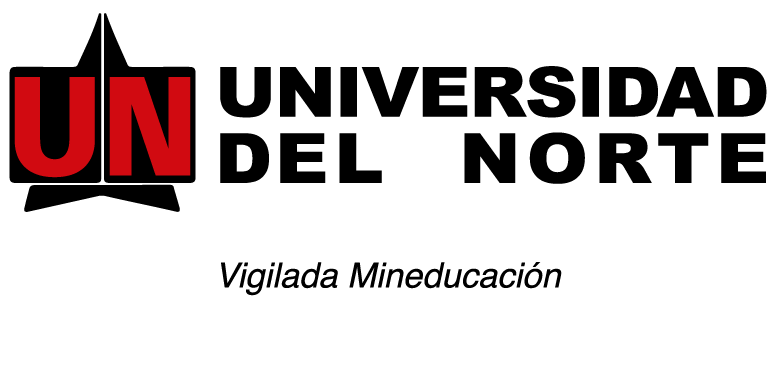
\includegraphics[scale=0.15]{UNWIDE.png} }{}


\begin{document}
	\title{
	\textbf{A characterization of Colombian industries under Schumpeter's patterns of innovation}
	}   
	
	\author[Taborda]{J.~Taborda\inst{1}}
	\institute[Uninorte]{\inst{1}Economics Student at 
		Universidad del Norte }
	\date[BA 2022-30]{Bachelor Thesis Progress. September 30th, 2022} 
	\begin{frame} 
		\titlepage 
	\end{frame}  

	\begin{frame}
		\frametitle{Table of Contents}
		\tableofcontents
	\end{frame}


	\AtBeginSection[]
	{
		\begin{frame}
			\frametitle{Table of Contents}
			\tableofcontents[currentsection]
		\end{frame}
	}
	
\section{Introduction}
	\begin{frame}[allowframebreaks]
		\frametitle{Introduction} 
		\begin{itemize}
			\item \textbf{Who drives innovation within an industry?}
			\item Could it be a small firm.... Or a large corporation?
			\item We will answer this question using Schumpeterian patterns of innovation --> \textbf{Mark I and II}
			\item How? Characterization --> Cluster analysis
			\item On the basis of...? EDIT and EAM
		\end{itemize}
	\end{frame}	
	\begin{frame}[allowframebreaks]
		\frametitle{Problem Statement}
		\begin{itemize}
			\item Characterization exercises "\textit{have been standing the test of time quite well}" (Fontana et al., 2012)
			\item Useful for policymaking
			\item But where do these exercises \textbf{take place}? 
			\item A gap in the literature for Colombia
		\end{itemize}
	\end{frame}
	\begin{frame}[allowframebreaks]
		\frametitle{Objectives}
		\begin{itemize}
			\item \textbf{Main objective}: \textbf{Characterize} industries in the Colombian manufacturing sector based on the framework of Schumpeter's Mark I and II, aiming to supply a better insight on the differences between industries by finding out what type of firm drives innovation.
			\framebreak
			\item \textbf{Specific Objectives:}
			\begin{itemize}
				\item \textbf{Utilize information} from the EDIT and EAM surveys to set up a database about firm features in manufacturing industries.
				\item Based on EDIT and EAM information, \textbf{construct a quantitative analysis} at the firm level that yields a result at the industry level, which in turn gives groundwork to create industry-level comparisons.
				\item Employing a cluster algorithm,\textbf{ group industry-level data} by common patterns and characterize them using Schumpeter's Mark I and II, which will give an insight into the drivers of innovation constrained to industrial structure and dynamics.
			\end{itemize}
		\end{itemize}
	\end{frame}
\section{Theory and background}
	\begin{frame}[allowframebreaks]
		\frametitle{Theoretical Framework}
		\begin{itemize}
			\item The concept of innovation (OECD, 2018)
			\begin{itemize}
				\item What is innovation?  (do not confuse with invention)
				
				\item \textit{\textbf{New or improved product or process (or a combination thereof) that differs significantly from the unit's previous
				products or processes and that has been made available to potential users (product) or brought into use by the unit (process)"	}}
				
				\item What is an innovative activity? (ACTI)
			\end{itemize}
		\end{itemize}
	\pagebreak
		\begin{itemize}
			\item Taxonomies of innovation
			\begin{itemize}
				\item By type: Market, process, product, etc... (OECD, 2018)
				\item By novelty and impact...
				\item Radical (Schumpeter, 1942)
				\item Incremental (Kirzner, 1973)
			\end{itemize}
		\end{itemize}
		\pagebreak
		\begin{itemize}
			\item Schumpeterian patterns of innovation
			\begin{itemize}
				\item Mark I: Schumpeter early thoughts. \textbf{Small firms are the drivers of innovation} (1911)
				\item Mark II: Schumpeter late deliberations. \textbf{Large firms are the drivers of innovation}, and perfect competition is not only inferior but inefficient.
			\end{itemize}
		\end{itemize}
		\pagebreak
		\begin{itemize}			
			\item \textbf{Mark I}: Perfect competition, \textbf{radical} innovations
			\item \textbf{Mark II}: Monopoly/Oligopoly, \textbf{incremental} innovations
			\item \textit{According to who}...? Market Structure and innovation:
			\begin{itemize}
				\item Fontana et al. (2012): Turbulence vs Stability
				\item Arrow replacement effect (1962)
				\item Baumol proposition (2004)
				\item Gilbert (2006) incentives to innovate based on potential profits
				\item Shapiro revisit (2012): Unifying principle... \textbf{competition}
			\end{itemize}
		\end{itemize}
	\end{frame}
\begin{frame}[allowframebreaks]
	\frametitle{Literature review}
	\begin{itemize}
		\item Previous works on the field: Malerba and Orsenigo (1996), Breschi et al. (2000), Landström \& Schön (2010), Castellaci and Zheng (2010), Corrocher et al. (2007).
		\item The Pavitt's alternative (1984). Which one is better? \textit{spoiler: depends}
		\begin{itemize}
			\item Pavitt: \textbf{Kondratiev waves} (Archibugi, 2001)
			\item Schumpeter: \textbf{Early/Late stages of an industry} (Malerba, 2005)
		\end{itemize}
	\end{itemize}
	\framebreak
	\begin{itemize}
		\item Not one size fits all
		\item Attempts in Colombia with Schumpeter? \textbf{Yes, but} not in characterization (Umaña-Aponte et al., 2013; Marroquín, 2010; Arroyo-Mina \& Guerrero, 2018; Langebaek-Rueda \& Vásquez, 2007).
		\item Attempts to characterize? \textbf{Yes, but} not with Schumpeter (Cerón et al., 2010; Ovallos-Gazabón \& Amar-Sepúlveda, 2014).
	\end{itemize}
\end{frame}

\section{Methodology}
	\begin{frame}[allowframebreaks]
	\frametitle{The Data}
	\begin{itemize}
		\item Cross-section
		\item Inner join of 2018 \textbf{EDIT} ("\textit{Encuesta de Desarrollo
		e innovación tecnológica}") and \textbf{EAM} (\textit{Encuesta Anual Manufacturera}) surveys by DANE (2019:2020)
		\item EAM is a \textbf{census}; EDIT samples EAM \textbf{industries} --> Inner join
		\item Criteria: Employees and profits
		\item Each firm has a \textit{"Numero de Orden}" (NORDEMP)
	\end{itemize}
	\pagebreak
	\begin{itemize}
		\item Number of observations: from almost 8000 to 6405
		\item I will employ variables that approach Breschi et al.
		(2000) and Malerba \& Orsenigo (1996) dimensions
		\item That means... \textbf{market concentration, stability and
		technological opportunities}
	\end{itemize}
	\framebreak
	\end{frame}
	\begin{frame}
	\begin{figure}
		\centering
		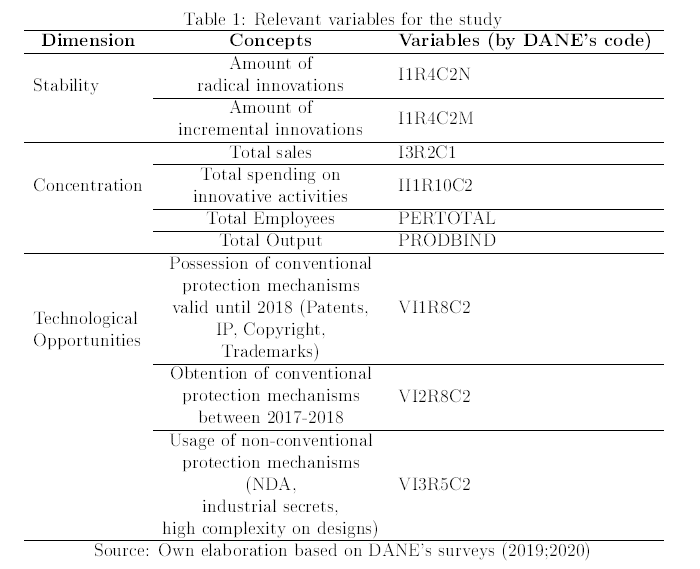
\includegraphics[scale=0.51]{table1.png}	
	\end{figure}
	\end{frame}
	
	\begin{frame}[allowframebreaks]
	\frametitle{The Measures}
	\begin{itemize}
		\item \textbf{Concentration (CON)}
		\item Based on Malerba and Orsenigo (1996) share on ACTI and sales
		\item Expanded to add supply share and labour share
	\end{itemize}
	\begin{equation}
		\centering
		CON = (HH_{ms}*HH_{msa}*HH_{lsd}*HH_{ss})^{1/4}
	\end{equation}
	\framebreak
		\begin{itemize}
		\item \textbf{Stability (STA)}
		\item The dynamic problem.\textbf{ EDIT is non comparable}
		\item Thus, we need another approach. A static approach
		\item Based on Baumol (2004) proposition
	\end{itemize}
	\begin{equation}
		\centering
		STA = Sr - Si
	\end{equation}
	\framebreak
	\begin{itemize}
		\item \textbf{Technological Opportunities (TO)}
		\item Based on Maleki et al. (2018) approach
		\item Growth rate of patents
		\item Non-comparability of EDIT --> Dynamic approach problem, again
		\item Static approach
	\end{itemize}
	\begin{equation}
		\centering
		TO = \dfrac{PM_{1718} + NCPM_{1718}}{PM}
	\end{equation}
	\end{frame}
	\begin{frame}[allowframebreaks]
		\frametitle{The Methods}
		\begin{itemize}
		\item \textbf{Important}: I had problems on industries with less than 20 observations. Some industries had 0 spending on ACTI. Hence, I establish 20 as the minimum number of observations in my study. \textbf{n = 5986}
		\pagebreak
		\item Method: k-means clustering
		\begin{itemize}
			\item 2 groups
			\item Lloyd algorithm
			\item 10 repetitions
		\end{itemize}
		\item \textbf{Where}? in \textcolor{cyan}{R}. \textit{pvclust}, \textit{factoextra} and \textit{stats}
		\pagebreak
		\item k-means in a nutshell (MacKay, 2003):
		\begin{itemize}
			\item \textit{Assignation phase}: Each observation gets assigned to the group with the closest mean (by Euclidean distance). Groups have a centroid
			\item \textit{Update phase}: Group parameters adjust to match the means of the data points.
			\item \textit{Repetition phase}: Assignation and Update phases repeat until they do not change anymore, that is, data points do not change their position in the groups.
		\end{itemize}
		\end{itemize}
	\end{frame}
\section{Preliminary Results}
	\begin{frame}
		 \begin{figure}[H]	
		 	\caption{Preliminary characterization of Colombian Manufacture using a two groups k-means clustering method}
		 	\centering
		 	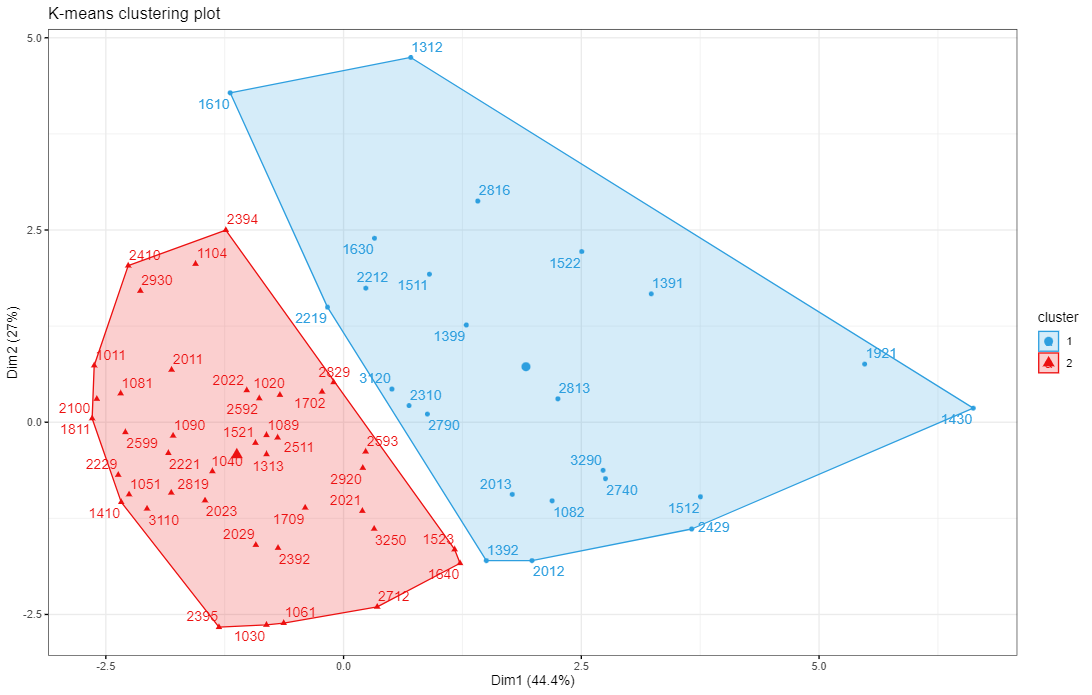
\includegraphics[scale = 0.29]{cluster.png}
		 \end{figure}
	\end{frame} 
	\begin{frame}
		\frametitle{Initial impressions}
		\begin{itemize}
			\item Dim1 and Dim2
			\item Two groups: Cluster Group 1 (CG1) and Cluster Group 2 (CG2)
			\item One is denser than the other
			\item Also, one has more firms than the other
				\begin{itemize}
					\item \textcolor{blue}{CG1} --> n = 794
					\item \textcolor{red}{CG2}  --> n = 5192
				\end{itemize}
		\end{itemize}
	\end{frame}
	\begin{frame}
		\frametitle{Descriptive statistics}
		\begin{figure}
			\centering
			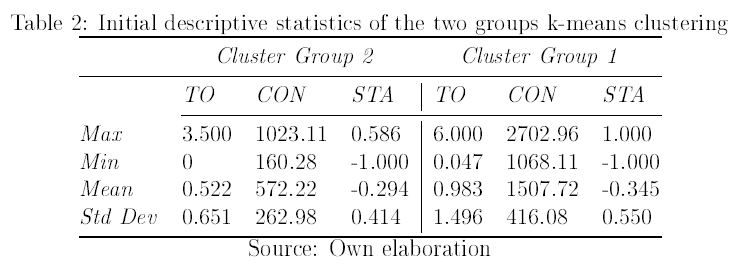
\includegraphics[scale=0.55]{descsta.png}
		\end{figure}
	\end{frame}
\section{Discussion}
	\begin{frame}[allowframebreaks]
		\begin{figure}
			\centering
			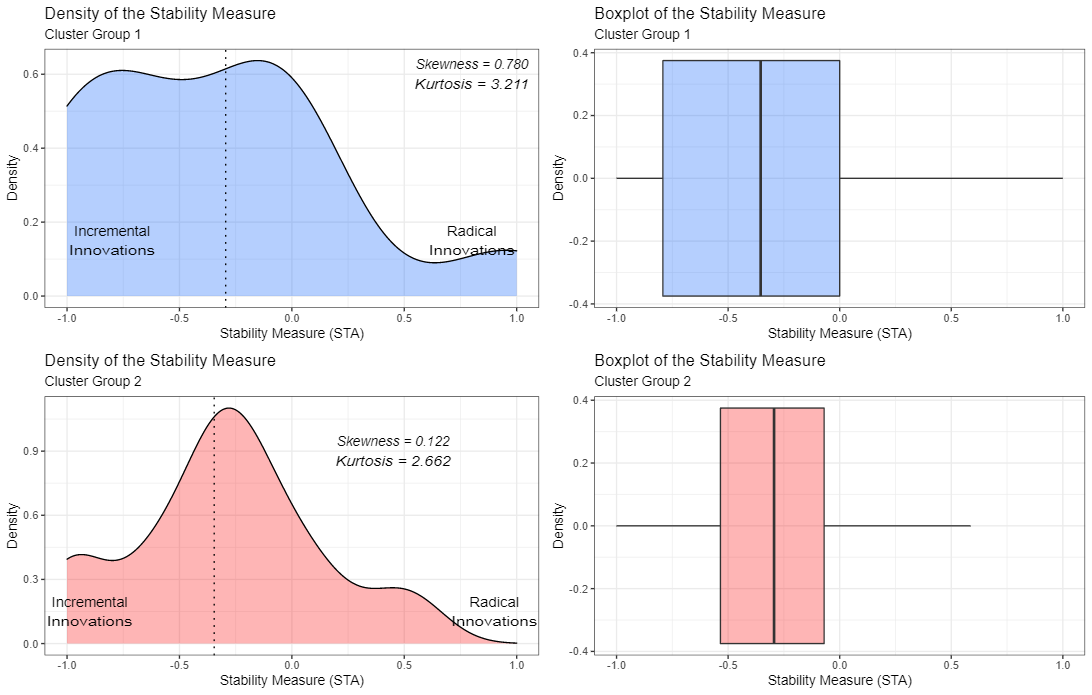
\includegraphics[scale=0.30]{sta.png}
		\end{figure}
	\framebreak
	\begin{figure}
		\centering
		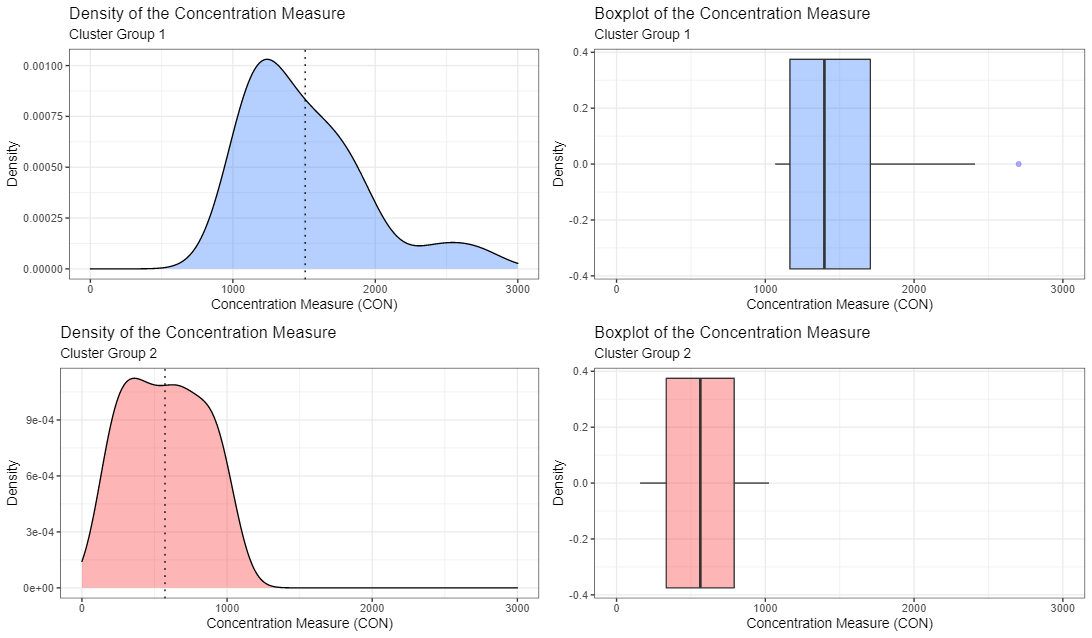
\includegraphics[scale=0.30]{pcon.png}
	\end{figure}
	\framebreak
	\begin{figure}
		\centering
		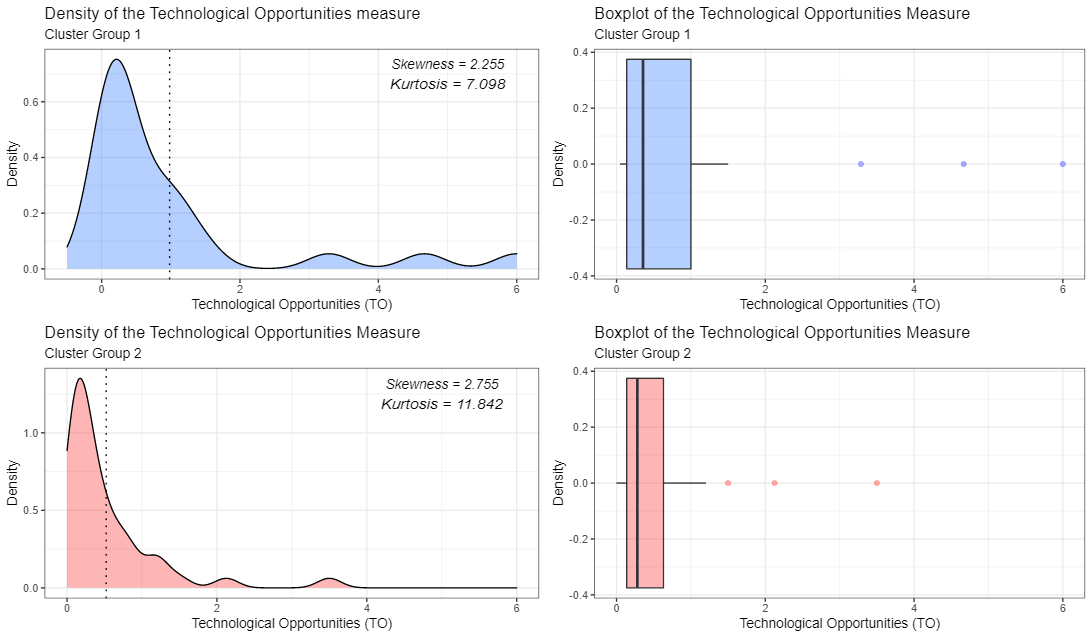
\includegraphics[scale=0.30]{to.png}
	\end{figure}
	\end{frame}
\section{Preliminary Conclusions}
	\begin{frame}[allowframebreaks]
		\frametitle{What can we conclude so far}
		\textbf{The most important conclusion!!...}
		\begin{itemize}
			\item \textcolor{red}{Red cluster} (CG2): Mark I industries
			\item \textcolor{blue}{Blue cluster} (CG1): Mark II industries
		\end{itemize}
	\framebreak 
		Moreover...
	\begin{itemize}
		\item We have been able to characterize Colombian industries under Schumpeterian patterns of innovation
		\item We found \textbf{Who drives innovation} --> On \textcolor{red}{Red cluster} (CG2), small firms drive innovation, but on \textcolor{blue}{Blue cluster} (CG1)...  it is all about large firms
		\item Concentration is the spearhead of our analysis, but our other two measures provide interesting results too
		\item Groundwork for policymaking and future studies
	\end{itemize}
	\end{frame}
\end{document}